\documentclass[11pt,a4paper,twoside]{article}
\usepackage[T1]{fontenc}
\usepackage[utf8x]{inputenc}
\usepackage{latexsym,amsfonts,amsmath,amsthm,amssymb, mathrsfs}
\usepackage{xcolor,bm, bbm}
\usepackage{amssymb}
\usepackage{tikz}
\usepackage{pgfplots}
\usetikzlibrary{patterns}

\begin{document}

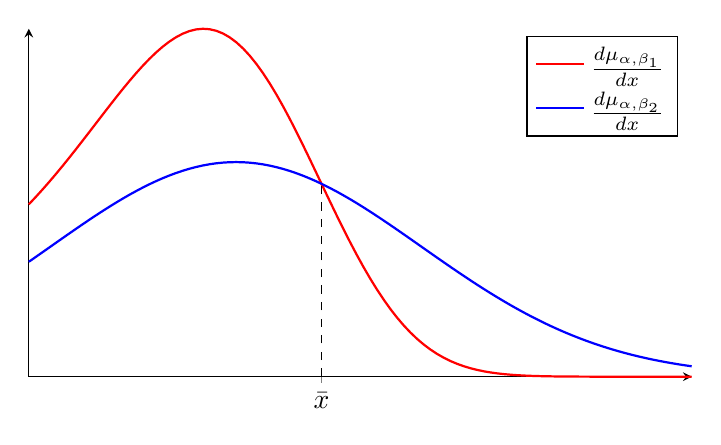
\begin{tikzpicture}
\begin{axis}[
clip=false,
    domain = 0:4, 
    samples = 100, 
    axis lines = left,
    width = 10cm,
    height = 6cm,
    ytick=\empty,
   xtick={1.76647}, 
   xticklabels={\(\bar{x}\)}
]
\addplot[red, thick, domain=0:4] {1.5*exp(-0.3*x^3 + x)};
\addplot[blue, thick, domain=0:4] {exp(-0.4*x^2 + x )};  
\legend{\(\frac{d \mu_{\alpha, \beta_1}}{dx}\), \( \frac{d \mu_{\alpha, \beta_2}}{dx}\)}

\end{axis}
\draw[dashed] (2.103*1.76647,0) -- (2.103*1.76647,1.5*1.67917);
\end{tikzpicture}

\end{document}